\documentclass[10pt]{article}
\usepackage[utf8]{inputenc}
\usepackage{geometry} % to change the page dimensions
\geometry{a4paper}
\usepackage{authblk}

%% Packages
\usepackage{graphicx, subcaption}
\usepackage{amsmath,amssymb,amsthm,amsfonts}
\usepackage{bm}
\usepackage{algorithm, algorithmic}
\usepackage{multirow}
\usepackage{bbm}
\usepackage{hyperref}
\usepackage{kotex}
\usepackage[labelformat=simple]{subcaption}

\usepackage{tikz}
\usetikzlibrary{shapes.geometric, arrows, positioning, calc}
\usetikzlibrary{backgrounds}
\usetikzlibrary{arrows.meta}

\tikzstyle{title} = [rectangle, minimum width=3cm, minimum height=1cm, text centered, draw=black, text width=3cm, fill=white!100]
\tikzstyle{startstop} = [rectangle, rounded corners, minimum width=3cm, minimum height=1cm,text centered, draw=black, fill=red!30]
\tikzstyle{io} = [trapezium, trapezium left angle=70, trapezium right angle=110, minimum width=3cm, minimum height=1cm, text width=1.3cm, text centered, draw=black, fill=blue!30]
\tikzstyle{process} = [rectangle, minimum width=3cm, text width=3cm, minimum height=1cm, text centered, draw=black, fill=orange!30]
\tikzstyle{decision} = [diamond, minimum width=3cm, minimum height=1cm, text centered, draw=black, fill=green!30]
\tikzstyle{arrow} = [thick,->,>=stealth]

\captionsetup[figure]{labelsep=period}
% \renewcommand{\thefigure}{\Roman{figure}}
% \captionsetup[subfigure]{labelformat=parens} % default is 'parens'
% \renewcommand{\thesubfigure}{\thefigure.\alph{subfigure}.}
\renewcommand\thesubfigure{(\alph{subfigure})}

%% Theorems
\theoremstyle{plain}
\newtheorem{theorem}{Theorem}[section]
\newtheorem{proposition}[theorem]{Proposition}
\newtheorem{lemma}[theorem]{Lemma}

\theoremstyle{remark}
\newtheorem{remark}[theorem]{Remark}
\newtheorem{example}[theorem]{Example}

\theoremstyle{definition}
\newtheorem{definition}[theorem]{Definition}

%% Equations
\numberwithin{equation}{section}

%% Algorithms
\renewcommand\algorithmicdo{}
\renewcommand\algorithmicthen{}
\renewcommand\algorithmicendfor{\textbf{end}}

%% Macros
\def\chfun{\mathbbm{1}}
\def\skel{\mathcal{S}}
\def\calc{\mathcal{C}}
\def\sko{\hat{\mathcal{S}}}
\def\ske{\mathcal{S}^8}
\def\endske{E\left(\mathcal{S}^8\right)}
\def\endomc{E\left(\Omega_c\right)}


\def\gphi{\nabla\phi}
\def\ngphi{\left|\nabla\phi\right|}
\def\ngphii{\left|\nabla\phi_i\right|}
\def\fci{F_{c,\,i}}
\def\fcj{F_{c,\,j}}
\def\cm{\, ,}
\def\pd{\, .}

\def\omi{\Omega_i}
\def\oma{\Omega_a}
\def\ome{\Omega_E}
\def\oms{\Omega_S}
\def\omc{\overline{\Omega}_P}
\def\omcc{\Omega_P}
\def\ER{\Omega_{Er}}

\def\sdf{\mbox{SDF}}

\DeclareMathOperator*{\argmax}{arg\,max}
\DeclareMathOperator*{\argmin}{arg\,min}
% \def\tOmega{\tilde{\Omega}}
% \def\tGamma{\tilde{\Gamma}}
% \def\tV{\tilde{V}}
% \def\W{\mathbb{W}}
% \def\tu{\tilde{u}}
% \def\bu{\bar{u}}
% \def\hu{\hat{u}}
% \def\bl{\bar{\lambda}}
% \def\p{\mathbf{p}}
% \def\P{\mathbf{P}}
% \def\intO{\int_{\Omega}}
% \def\intOs{\int_{\Omega_s}}
% \def\m{\mathbf{m}}
% \def\n{\mathbf{n}}
% \def\blambda{\bm{\lambda}}

% \def\tE{\tilde{E}}
% \def\N{\mathcal{N}}

% \def\div{\mathrm{div}}
% \def\proj{\mathrm{proj}}
% \def\prox{\mathrm{prox}}
% \def\ran{\mathrm{ran}\,}
% \def\ed{\mathrm{ed}}
% \def\supp{\mathrm{supp}\,}
% \def\TOL{\mathrm{TOL}}
% \DeclareMathOperator*{\argmin}{\arg\min}

% Text Color and Strike
\usepackage[normalem]{ulem}
\usepackage{color}
\newcommand{\red}[1]{{\color{red}{#1}}}
\newcommand{\blue}[1]{{\color{blue}{#1}}}

\title{ Individual Tooth Segmentation in Human Teeth Image by Pre--Edge Region Learning }
\author{Seongeun Kim and Chang-Ock Lee}
\affil{Department of Mathematical Sciences, KAIST, Daejeon 34141, Korea}
\date{ }

\begin{document}
\maketitle

\begin{abstract}
Segmentation of individual tooth region in a human teeth image have been performed well on CT or X-ray images. However, in human teeth images taken outside the oral cavity, it is difficult to segment individual tooth due to common obstacles such as weak edges, intensity inhomogeneities and strong light reflections. In this work, we propose a method for segmenting individual teeth from a human teeth image. The key of the method is to obtain the pre--edge region using the deep supervised learning method. To avoid spending time and cost in the labeling process, we present a strategy to support the labeling process using existing model--based methods.

In a recent work \cite{WU:2016}, a 3D model reconstruction method in a single teeth image using individual tooth boundaries was proposed, which emphasizes the importance of segmentation of tooth regions.
\end{abstract}

{\small \textbf{Key words}
Tooth segmentation, Pre--edge region, Supervised Learning, Image Segmentation, Geometric attraction--driven flow, Edge region, Weak edge, Light reflection, Multiple level set functions}

{\small \textbf{AMS subject classifications}
94A08, 68T07}

%% Main text starts ---------------------------------------------------------------------------------------------------
% Section: Introduction
\section{Introduction}
\label{Sec:Introduction}

The image segmentation is one of major topic in the field of computer vision. The main goal of image segmentation is to segment objects in an image according to a specific purpose and many outstanding methodologies have been developed. The active contour model is one of the popular methods for the image segmentation. It makes the contour surrounding an object move to the boundary of the objects with the designed force \cite{Kass:1988:Snakes}; The gradient vector flows \cite{Xu:1997:GVF}, geodesic active contours \cite{Caselles:1997:GAC} and balloon forces \cite{Cohen:1991:Balloon} are generally well-known models with different forces. There are also variational models that uses statistical information of intensities
in an image \cite{Park:2014:SRM,Zhu:1996:RegCompet}. In \cite{Chan:2001:chanvese}, unlike the previous methods using edge maps, a region-based active contour method has been proposed.

Segmentation of individual tooth in human teeth images have mainly been performed in computed tomography (CT) or X-ray images \cite{Yuan:2020:teethParanomic,Naumovich:2015:teethCT3D,Said:2006:teethxray,Shah:2006:teethautoseg}. The CT or X-ray images are grayscale, and the tooth regions are easily segmented because the intensities of teeth region are much stronger than the gums or tissues. But segmentation of individual tooth in a camera taken teeth image is a more difficult problem. In the teeth images, weak edges and light reflections appear and even the colors and illuminance are inhomogeneous because of plaques and the oral structure. These obstacles make it difficult to segment individual tooth in a teeth image. Several attempts have been made to segment individual tooth in a teeth image. In \cite{LeeWater:2010, LeeColor:2009} the watershed algorithm with color information was proposed. In \cite{LeeSegRemoval:2010}, an additional light reflection removal process \cite{LeeRemoval:2010} was applied before segmentation. In recent studies \cite{Kim:2020,Pham:2020,Zhu:2020:teethMaskrcnn}, segmentations using deep learning methods with Mask R-CNN \cite{He:2018:MRCNN} were proposed.

Individual tooth segmentation can be applied to reconstruction of 3D teeth model. In \cite{Yuan:2020:teethParanomic,Naumovich:2015:teethCT3D}, 3D teeth is reconstructed by segmentation in CT teeth image. In \cite{WU:2016}, a 3D teeth model reconstruction using a teeth image was proposed. Here, the 3D teeth model reconstruction is achieved using individual tooth boundaries in a teeth image. In here, a supervised learning method BEL \cite{Dollr:2006} was used to extract the individual tooth boundaries with manually labeled $40$ teeth studio-taken images as the training data. 

Existing methodologies can be divided into two categories; model based method or supervised learning method. Model--based methods focus on segmentation using the color information. This methods can be expected to produce poor results when applied to images obtained in an unrefined environment. On the other hand, it is well known that a supervised learning methods can give outstanding results, but it takes a lot of time and effort in the labeling process for the learning. In this paper, we segment individual tooth regions by obtaining pre--edge region using the supervised learning method. In the supervised learning process, data labeling is assisted by model--based method. 

The remainder of this paper is organized as follows. In Section~\ref{Sec:er_teeth}, we will talk about GADF, edge regions, and the problems of edge regions obtained from teeth images. In Section~\ref{Sec:PM}, the proposed algorithm is described and the experimental results are present in Section~\ref{Sec:result}. We will conclude this paper at Section~\ref{Sec:Conclusion}. 

% Sec:Background
\section{Edge regions in human teeth image}
\label{Sec:er_teeth}
In this section, we briefly review geometric attraction-driven flow (GADF) \cite{Hahn:2006, Hahn:2010:GADF} and edge region, which play key role in segmenting individual tooth. Concerning the problematic features of the teeth image we will show problems of edge region obtained directly from GADF.

% Subsec:GADF
\subsection{Geometric Attraction-Driven Flow}
\label{Subsec:GADF}
Let $I\colon\Omega\subset\mathbf{R}^2\rightarrow[0,\,1]$ be a given smooth gray image. The image intensity changes rapidly on the boundary of objects in the image. Thus, a point $x\in\Omega$ is defined as an edge of the image if
\begin{align}
    u_x''(0)=0\cm \label{Def:edge}
\end{align}
where
\begin{align*}
    u_x(s) = I\left( x + s\frac{\nabla{I(x)}}{|\nabla{I(x)}|} \right)\pd
\end{align*}
In \cite{Hahn:2010:GADF}, the GADF is defined as
\begin{align}
    F_a(x) = \mbox{sgn}(\ell(x))\frac{\nabla I(x)}{\left|\nabla{I(x)}\right|},\quad \forall{x}\in\Omega\cm  \label{Def:gadf}
\end{align}
where $\mbox{sgn}$ is the sign function and 
\begin{align*}
    \ell(x) &= \int^{\epsilon}_{0} {u'_x(s)}\,ds - \int^{0}_{-\epsilon} {u'_x(s)}\,ds\quad\mbox{for a small}~\epsilon > 0\pd
\end{align*}
By the definition, $F_a(x)$ points along the line $x + s\frac{\nabla{I(x)}}{|\nabla{I(x)}|}$ towards the edge where $u_x''(s)=0$. 

Under this setting, contour evolution using a level set formulation is proposed in \cite{Hahn:2010:GADF}:
\begin{align}
    \frac{\partial}{\partial{t}}\phi(x,\,t) &= \mu\kappa(\phi)\left|\nabla\phi\right| - \chi_{\oma}F_a\cdot\nabla\phi + \chi_{\Omega_b}F_b|\nabla\phi|\cm \label{Eq:gadf}\\
    \phi(x,\,0) &= \phi_0(x)\cm \nonumber
\end{align}
where $\mu$ is a constant, $\phi_0$ is the initial $\sdf$ and $\oma$ is a region in which $F_a$ faces each other, i.e.,
\begin{align}
    \Omega_a = \delta_{S}\left( \Omega_E \right)\cm \label{Def:oma}
\end{align}
where
\begin{align*}
    \Omega_E = \left\{ x\in\Omega \mid F_a(x^*) \cdot F_a(x) < 0 ~\mbox{and}~ x^*=x+F_a(x) \right\}\pd %\label{Def:pre_er}
\end{align*}
and $\delta_{S}(X)$ is a dilation of a set $X$ by a structuring element $S$ which is $3\times3$ matrix with origin at the center. Observe that the initial contour goes outward in $\Omega_b = \Omega\setminus\Omega_a$ by a balloon force $F_b$ and approaches the edge by $F_a$ once it reaches in $\Omega_a$.

The edge region is a region that is thought to contain edges. Since $\oma$ contains all edges by the definition, it can be a first candidate of the edge region. In fact, whole region of $\oma$ is used as an edge region in \eqref{Eq:gadf}. But, in practice $\oma$ contains a lot of unnecessary parts, and so it cannot be used as an edge region directly.

% Subsection: Edge regions outside the tooth boundaries
\subsection{Edge regions outside the tooth boundaries}
\label{Subsec:er_outside}

그림으로 설명을 대체?
In human teeth images, weak edges are appeared at the boundary between teeth and gums, the boundary between two teeth with similar color and brightness, and the junction of boundaries. It is hard to extract those weak edges using existing methods but $\oma$ in \eqref{Def:oma} contains all edges in an image \cite{Hahn:2010:GADF} including weak edges. On the other hand, $\oma$ contains unnecessary parts outside the tooth boundaries due to inhomogeneity of the object surface or noise in the image. Due to these edges, $\oma$ includes many connected regions outside the tooth boundary as shown in Figure~\ref{Fig:1d}.
% Figure: Weak edges in teeth image
\begin{figure}
    \centering
    \begin{subfigure}{1\textwidth}
        \centering
        \includegraphics[width=10cm]{./Figures/Fig1_img.png}
        \caption{A whole teeth image}
        \label{fig:1a}
    \end{subfigure} 
    \newline 
    
    \vspace{1mm}
    
    \begin{subfigure}{.18\textwidth}
        \centering
        \includegraphics[width=2.6cm]{./Figures/Fig1_img1.png}
        \includegraphics[width=2.6cm]{./Figures/Fig1_img3.png}
        \includegraphics[width=2.6cm]{./Figures/Fig1_img2.png}
        \caption{}
    \end{subfigure}
    \begin{subfigure}{.18\textwidth}
        \centering
        \includegraphics[width=2.6cm]{./Figures/Fig1_sbl1.png}
        \includegraphics[width=2.6cm]{./Figures/Fig1_sbl3.png}
        \includegraphics[width=2.6cm]{./Figures/Fig1_sbl2.png}
        \caption{Sobel}
    \end{subfigure}
    \begin{subfigure}{.18\textwidth}
        \centering
        \includegraphics[width=2.6cm]{./Figures/Fig1_cny1.png}
        \includegraphics[width=2.6cm]{./Figures/Fig1_cny3.png}
        \includegraphics[width=2.6cm]{./Figures/Fig1_cny2.png}
        \caption{Canny}
    \end{subfigure}
    \begin{subfigure}{.18\textwidth}
        \centering
        \includegraphics[width=2.6cm]{./Figures/Fig1_er1.png}
        \includegraphics[width=2.6cm]{./Figures/Fig1_er3.png}
        \includegraphics[width=2.6cm]{./Figures/Fig1_er2.png}
        \caption{$\ome$}
        \label{Fig:1d}
    \end{subfigure}
    \caption{(a) A image and (b) sub-images in the green boxes. The results of various methods are shown. (c--d) Sobel and Canny edge detectors with automatically chosen thresholds by MATLAB. (e) $\Omega_E$ from the GADF. As shown in the resulting images, GADF can detect tooth boundaries much better than the other methods. However, there are many more unnecessary regions than the others. }
    \label{Fig:weak_edges}
\end{figure}
They can be roughly divided into three categories according to the causes:
\begin{itemize}
    \item [(C--1)] Noise or small stains,
    \item [(C--2)] Large stains with unclear boundary,
    \item [(C--3)] Strong light reflections.
\end{itemize} 
The connected components of $\oma$ generated by the tooth boundary are large and intensities of the image change rapidly around them, thus we preferentially removed opposite regions; the regions with small size or flat image intensities \cite{Hahn:2006}. Since the size of regions caused by small stains are also small and intensities around regions caused by noise are flat, the regions caused by (C--1) are easily removed. 


하나로 묶어서 설명?
Some stains on the image makes a large edge region. The region caused by stain with clean boundary forms closed shape following the boundary of the stain. But if the boundary of stain is not all clean, then breakings or fragments are occurs on the stain. As the initial contour evolves, these breakings and fragments can be disregarded by using the curvature term. Thus (C--2) . 

The regions resulting from (C--3) are large and of a closed shape. Because of the shape without ends, it cannot be processed like (C--2). These edge regions, like a barrier, block the movement of the contour and make it difficult to find the correct tooth boundary. As a result, they are major obstacles to individual tooth segmentation. The contour evolution around the regions of various shapes is shown in Figure~\ref{Fig:er_outside}.

% Figure: Edge regions outside the tooth boundaries
\begin{figure}
    \centering
    % First row
    \begin{subfigure}{.24\textwidth}
        \centering
        \includegraphics[height=2.8cm]{./Figures/Fig2_img.png}
        \caption{}
        \label{Fig:2a}
    \end{subfigure}
    \begin{subfigure}{.24\textwidth}
        \centering
        \includegraphics[height=2.8cm]{./Figures/Fig2_er.png}
        \caption{$\ome$}
        \label{Fig:2b}
    \end{subfigure}
    \begin{subfigure}{.24\textwidth}
        \centering
        \includegraphics[height=2.8cm]{./Figures/Fig2_reser.png}
        \caption{}
        \label{Fig:2c}
    \end{subfigure}\\
    \vspace{1mm}
    % First row
    \begin{subfigure}{.025\textwidth}
        \centering
        \caption*{\rotatebox[origin=c]{90}{\hspace{-4mm} (d) Left tooth}}
    \end{subfigure}
    \begin{subfigure}{.18\textwidth}
        \centering
        \includegraphics[height=2.4cm]{./Figures/Fig2_evolve_1/iter0.png}
    \end{subfigure}
    \begin{subfigure}{.18\textwidth}
        \centering
        \includegraphics[height=2.4cm]{./Figures/Fig2_evolve_1/iter150.png}
    \end{subfigure}
    \begin{subfigure}{.18\textwidth}
        \centering
        \includegraphics[height=2.4cm]{./Figures/Fig2_evolve_1/iter250.png}
    \end{subfigure}
    \begin{subfigure}{.18\textwidth}
        \centering
        \includegraphics[height=2.4cm]{./Figures/Fig2_evolve_1/iter300.png}
    \end{subfigure}
    \begin{subfigure}{.18\textwidth}
        \centering
        \includegraphics[height=2.4cm]{./Figures/Fig2_evolve_1/iter1000.png}
    \end{subfigure}\\
    \vspace{1mm}
    % Second row
    \begin{subfigure}{.025\textwidth}
        \centering
        \caption*{\rotatebox[origin=c]{90}{\hspace{-4mm} (e) Right tooth}}
    \end{subfigure}
    \begin{subfigure}{.18\textwidth}
        \centering
        \includegraphics[height=2.4cm]{./Figures/Fig2_evolve_2/iter0.png}
    \end{subfigure}
    \begin{subfigure}{.18\textwidth}
        \centering
        \includegraphics[height=2.4cm]{./Figures/Fig2_evolve_2/iter200.png}
    \end{subfigure}
    \begin{subfigure}{.18\textwidth}
        \centering
        \includegraphics[height=2.4cm]{./Figures/Fig2_evolve_2/iter350.png}
    \end{subfigure}
    \begin{subfigure}{.18\textwidth}
        \centering
        \includegraphics[height=2.4cm]{./Figures/Fig2_evolve_2/iter650.png}
    \end{subfigure}
    \begin{subfigure}{.18\textwidth}
        \centering
        \includegraphics[height=2.4cm]{./Figures/Fig2_evolve_2/iter1000.png}
    \end{subfigure}\\
    \vspace{1mm}
    % Third row
    \begin{subfigure}{.025\textwidth}
        \caption*{\rotatebox[origin=c]{90}{\hspace{-3mm} (f) Outside}}
    \end{subfigure}
    \begin{subfigure}{.18\textwidth}
        \centering
        \includegraphics[height=2.4cm]{./Figures/Fig2_evolve_3/iter0.png}
    \end{subfigure}
    \begin{subfigure}{.18\textwidth}
        \centering
        \includegraphics[height=2.4cm]{./Figures/Fig2_evolve_3/iter200.png}
    \end{subfigure}
    \begin{subfigure}{.18\textwidth}
        \centering
        \includegraphics[height=2.4cm]{./Figures/Fig2_evolve_3/iter350.png}
    \end{subfigure}
    \begin{subfigure}{.18\textwidth}
        \centering
        \includegraphics[height=2.4cm]{./Figures/Fig2_evolve_3/iter650.png}
    \end{subfigure}
    \begin{subfigure}{.18\textwidth}
        \centering
        \includegraphics[height=2.4cm]{./Figures/Fig2_evolve_3/iter1000.png}
    \end{subfigure}\\

    \caption{(a) Teeth image with light reflection. (c) Results obtained from (b) by removing regions caused by (C-1) and with dilation. (d--f) From left to right, the contour evolution over time by \eqref{Eq:gadf} over time is shown. The first column shows initial contours located at (d) the left tooth, (e) the right tooth, and (f) outside of teeth. Observe that the contour goes into the narrow area of (c), but does not the large, closed regions and finally stops. Especially in (d), the contour cannot reach the entire tooth boundary. }
    \label{Fig:er_outside}
\end{figure}

% Subsection: Avoidance of light reflections in the teeth image
\subsection{Avoiding light reflections in teeth images}
\label{Subsec:avoidance}

There are previous studies to remove light reflections in a single image \cite{SpecRemoval:2018,SpecRemoval:2020,SpecRemoval:2016,SpecRemoval:2015}. In these, an image was separated into reflective region and non--reflective region, using intensity histogram or assuming a dichromatic image model. These methods are based on color information of the reflective region, but in the case of teeth images, the colors of the light reflection and the tooth surface are almost the same due to the characteristics of human teeth. For this reason, when these methods are actually applied, parts of the tooth surface is also removed with the light reflection. 

There has been an attempt to remove the light reflection in teeth images using the single layer perceptron \cite{LeeRemoval:2010}, but there is a limitation that it cannot be applied to a wide range of image because learning is processed using only one image as well as the perceptron has an extremely simple structure.

The most important thing is that even if light reflection is removed from the teeth image, individual tooth can not be segmented immediately. There are a lot of unnecessary edges appear other than due to the light reflection. Each is easily breakable, but if they stick together forming a large bunch or form a closed area by connecting to the tooth boundary, it becomes an obstacle to boundary detection. In addition, if light reflection appears on the tooth boundary, the edge collapses when the light reflection is removed, making the boundary undetectable. Therefore, we seek a way to directly obtain only the edge region near the tooth boundary, regardless of stains, noise or light reflection of the image. For this, a supervised learning method with deep neural networks is considered.

% Section: Proposed Method
\section{Proposed Method}
\label{Sec:PM}
In this section, we describe the steps of the proposed individual tooth segmentation algorithm. It have the following four main steps and the whole process is shown in Figure~\ref{Fig:flowchart}:

\begin{itemize}
    \item[STEP 1] Obtaining pre-edge regions from a neural network,
    \item[STEP 2] Refinement of the pre-edge region,
    \item[STEP 3] Segmentation using active contours with competing ballon forces,
    \item[STEP 4] Identification of tooth and non-tooth region.
\end{itemize}

% Figure: Algorithm flowchart
\begin{figure}
    \centering
    \begin{subfigure}[]{1\textwidth}
        % \centering
        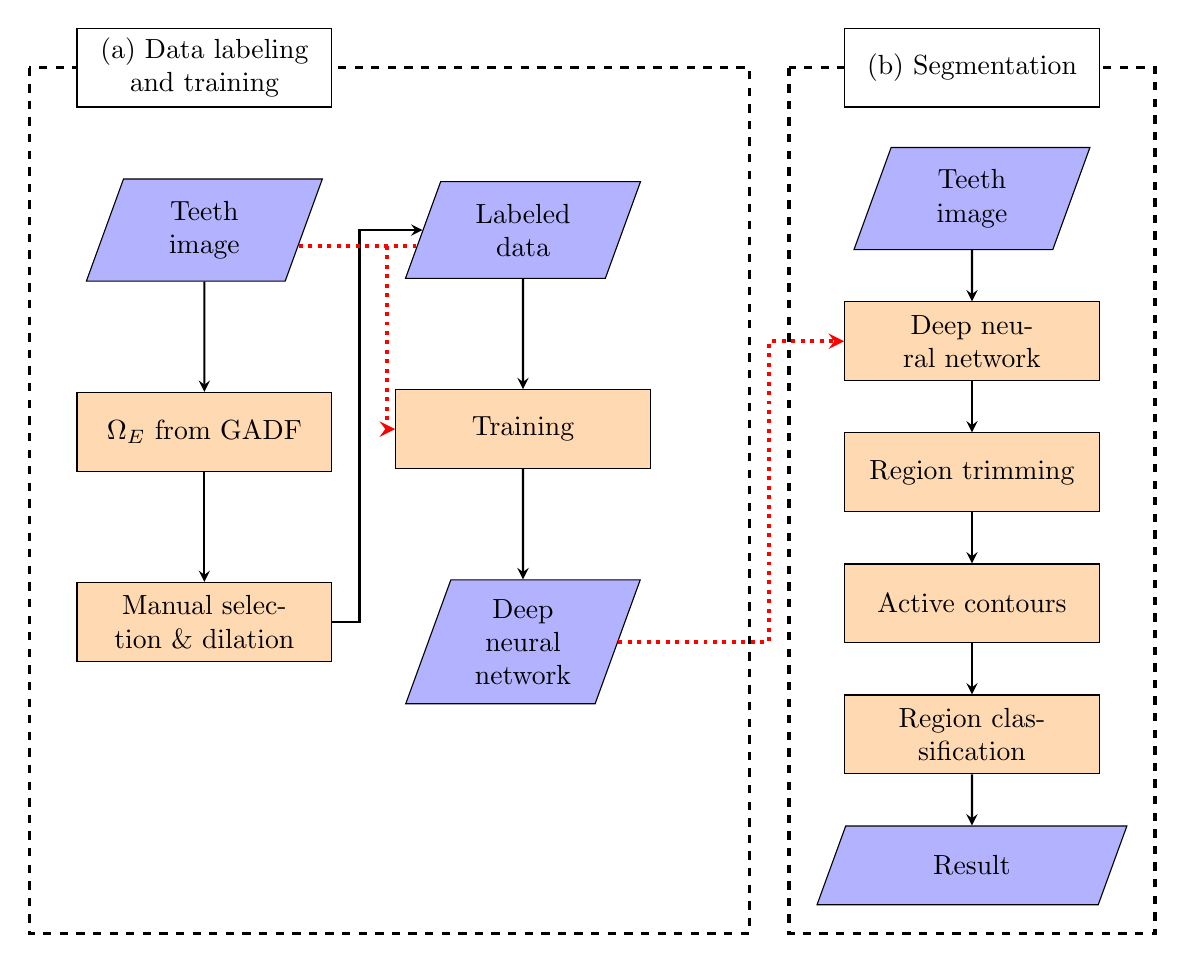
\begin{tikzpicture}[node distance=1.4cm and 1.5cm]
            \node (title1) [title] {(a) Data labeling and training};
            \node (title3) [title, right=6.5cm of title1] {(b) Segmentation};
            \node (teeth1) [io, below=.9cm of title1] {Teeth image};
            \node (pro11) [process, below=of teeth1] {$\Omega_E$ from GADF};
            \node (pro12) [process, below=of pro11] {Manual selection \& dilation};
            \node (label) [io, right=of teeth1] {Labeled data};
            \node (pro14) [process, below=of label] {Training};
            \node (dnn) [io, below=of pro14] {Deep neural network};
            
            \node (teeth3) [io, below=.5cm of title3] {Teeth image};
            \node (pro31) [process, below=.65cm of teeth3] {Deep neural network};
            \node (pro32) [process, below=.65cm of pro31] {Region trimming};
            \node (pro33) [process, below=.65cm of pro32] {Active contours};
            \node (pro34) [process, below=.65cm of pro33] {Region classification};
            \node (res) [io, below=.65cm of pro34] {Result};
            
            \draw [arrow] (teeth1) -- (pro11);
            \draw [arrow] (pro11) -- (pro12);
            \draw [arrow] (pro12.east) -| ($(label.west) + (-.8, 0)$) -- (label.west);
            \draw [arrow] (label) -- (pro14);
            \draw [arrow] (pro14) -- (dnn);
            \draw [arrow] (teeth3) -- (pro31);
            \draw [arrow] (pro31) -- (pro32);
            \draw [arrow] (pro32) -- (pro33);
            \draw [arrow] (pro33) -- (pro34);
            \draw [arrow] (pro34) -- (res);

            \draw [red,line width=.5mm,dotted] ($(teeth1.east) + (-.07, -.2)$) |- ($(label.west) + (-.07, -.2)$);
            \draw [arrow, red,line width=.5mm, dotted] ($(label.west) + (-.45, -.2)$) |- (pro14.west);
            \draw [arrow, red,line width=.5mm, dotted] (dnn.east) -| ($(pro31.west) + (-.95,0)$) -- (pro31.west);
            \begin{scope}[on background layer]
                \draw[black,line width=.4mm,dashed] ($(title1.west)+(-.6,0)$)  rectangle ($(title1.east)+(5.3,-11)$);
                \draw[black,line width=.4mm,dashed] ($(title3.west)+(-.7,0)$)  rectangle ($(title3.east)+(.7,-11)$);
            \end{scope}
        \end{tikzpicture}
    \end{subfigure}
    \caption{Algorithm flowchart; (a) data labeling and training process (b) segmentation process.}
    \label{Fig:flowchart}
\end{figure}
    
% Subsection: Obtaining pre-edge regions from a neural network
\subsection{Obtaining pre-edge regions from a neural network}
\label{Subsec:pre_er}

As shown in Figure~\ref{Fig:flowchart}(a), we make labels for training data using GADF and manual selection; first, we manually select the connected components of $\Omega_E$ overlapping the tooth boundary, and the label $Y\colon\Omega\subset\mathbf{R}^2\rightarrow\{0,\,1\}$ is defined as a binary function
\begin{align*}
    Y(x) =
    \begin{cases}
        1 & x\in\oms\\
        0 & \mbox{otherwise}
    \end{cases}\cm
\end{align*}
where $\oms$ is obtained by dilation of the selected region from $\ome$ by a structuring element that is an $\omega\times\omega$ matrix with the origin at the center. For training, the part of ResNeSt--50 \cite{Zhang:2020} before the global average pooling layer is used as the encoder part, and a custom upscale module is designed for the decoder part. The network takes a 3 channel image as an input $X\colon\Omega\rightarrow\mathbf{R}^3$ and produces a 1 channel image $\hat{Y}\colon\Omega\rightarrow(0,\,1)$ and is trained by minimizing the binary cross entropy (BCE) loss function \cite{Zhang:2018:BCE}. In Figure~\ref{Fig:labeling}, the labeling process is presented and the entire network structure is shown in the Figure~\ref{Fig:network}.

% Figure: Labeling images
\begin{figure}[]
    \centering
    \begin{subfigure}[]{.4\textwidth}
        \centering
        \includegraphics[height=3.8cm]{./Figures/Fig4_img.png}
        \caption{}
        \label{Fig:4a}
    \end{subfigure}
    \begin{subfigure}[]{.4\textwidth}
        \centering
        \includegraphics[height=3.8cm]{./Figures/Fig4_er.png}
        \caption{$\ome$}
        \label{Fig:4b}
    \end{subfigure}\\
    \vspace{1mm}
    \begin{subfigure}[]{.4\textwidth}
        \centering
        \includegraphics[height=3.8cm]{./Figures/Fig4_seler.png}
        \caption{$\Omega_s$}
        \label{Fig:4c}
    \end{subfigure}
    \begin{subfigure}[]{.4\textwidth}
        \centering
        \includegraphics[height=3.8cm]{./Figures/Fig4_label.png}
        \caption{labeled image}
        \label{Fig:4d}
    \end{subfigure}
    \caption{ Labeling process described in Section~\ref{Subsec:pre_er}. (a) An image in the training dataset. (b) The region $\Omega_E$. (c) Manually selected regions. (d) The labeled image obtained from (c) by dilation. }
    \label{Fig:labeling}
\end{figure}

The network output $\hat{Y}(x)$ is the probability of an edge region caused by tooth boundary exists at $x$. We call
\begin{align*}
    \omcc = \left\{ x\in\Omega \mid \hat{Y}(x) > 0.5 \right\}
\end{align*}
as a pre--edge region of $X$, and some pre--edge regions are shown in Figure~\ref{Fig:pre_er}. One notable point is that although the label contains many unnecessary regions, most of $\omcc$ are correctly located on the tooth boundary.

% Figure: Network structure
\begin{figure}[]
    \centering
    \begin{subfigure}[]{1\textwidth}
    \newcommand*{\al}{0.3}%
    \newcommand*{\aw}{1.mm}%
    \newcommand*{\hei}{1.1 cm}%
    \newcommand*{\flr}{3.5cm}%
    \newcommand*{\wgap}{1cm}%
    \newcommand*{\init}{0}%
    \newcommand*{\wwa}{.2}%
    \newcommand*{\wwb}{.3}%
    \newcommand*{\wwc}{.4}%
    \newcommand*{\wwd}{.5}%
    \newcommand*{\wwe}{.6}%
    \newcommand*{\wwf}{.7}%
    \newcommand*{\wwg}{.9}%

    \newcommand*{\hha}{1}%
    \newcommand*{\hhb}{.9}%
    \newcommand*{\hhc}{.8}%
    \newcommand*{\hhd}{.6}%
    \newcommand*{\hhe}{.4}%
    \newcommand*{\hhf}{.2}%
    \newcommand*{\hhg}{.2}%
    \centering
    \begin{tikzpicture}[]
        \footnotesize
        \node (x0) at (0,0) [draw=none,minimum width=1mm,minimum height=\hei, fill=blue!50!white,label=above:{$3$}] {};
        \draw [-{Triangle[scale=.5]},line width=\aw,color=red!70!black] (x0.south) to ++(0,-\al);

        \node (x1) at ($(x0) + (0,-\hei-\al cm - .3 cm)$) [draw=none,minimum width=\wwa cm,minimum height=\hhb*\hei, fill=blue!50!white,label=above:{$32$}] {}; 
        \draw [-{Triangle[scale=.5]},line width=\aw,color=orange!80!white] (x1.east) -- ++(\al, 0);

        \node (x2) at ($(x1) + (\al+ \wwa/2 + \wwa/2,0)$) [draw=none,minimum width=\wwa cm,minimum height=\hhb*\hei, fill=blue!50!white,label=above:{$32$}] {};
        \draw [-{Triangle[scale=.5]},line width=\aw,color=orange!80!white] (x2.east) -- ++(\al, 0);
        
        \node (x3) at ($(x2) + (\al+\wwa/2 + \wwb/2,0)$) [draw=none,minimum width=\wwb cm,minimum height=\hhb*\hei, fill=blue!50!white,label=above:{$64$}] {};
        \draw [-{Triangle[scale=.5]},line width=\aw,color=yellow!80!black] (x3.south) to ++(0,-\al);
        
        \node (x4) at ($(x3) + (0,-\hhb*\hei-\al cm - .3 cm)$) [draw=none,minimum width=\wwb cm,minimum height=\hhc*\hei, fill=blue!50!white,label=above:{$64$}] {};
        \draw [-{Triangle[scale=.5]},line width=\aw,color=green!80!black] (x4.east) -- ++(\al, 0);
        
        \node (x5) at ($(x4) + (\al+\wwb/2 + \wwd/2,0)$) [draw=none,minimum width=\wwd cm,minimum height=\hhc*\hei, fill=blue!50!white,label=above:{$256$}] {};
        \draw [-{Triangle[scale=.5]},line width=\aw,color=green!80!black] (x5.east) -- node [above, color=black] {$\times 2$} ++(1.5*\al, 0);

        \node (x6) at ($(x5) + (1.5*\al+\wwd/2 + \wwd/2,0)$) [draw=none,minimum width=\wwd cm,minimum height=\hhc*\hei, fill=blue!50!white,label=above:{$256$}] {};
        \draw [-{Triangle[scale=.5]},line width=\aw,color=cyan!90!green] (x6.south) to  ++(0,-\al) {};

        \node (x7) at ($(x6) + (0,-\hhc*\hei-\al cm - .3 cm)$) [draw=none,minimum width=\wwe cm,minimum height=\hhd*\hei, fill=blue!50!white,label=above:{$512$}] {};
        \draw [-{Triangle[scale=.5]},line width=\aw,color=cyan!90!green] (x7.east) to node [above, color=black] {$\times 3$} ++(1.5*\al,0) {};

        \node (x8) at ($(x7) + (1.5*\al+\wwe/2 + \wwe/2,0)$) [draw=none,minimum width=\wwe cm,minimum height=\hhd*\hei, fill=blue!50!white,label=above:{$512$}] {};
        \draw [-{Triangle[scale=.5]},line width=\aw,color=blue!60!black] (x8.south) to  ++(0,-\al) {};

        \node (x9) at ($(x8) + (0,-\hhd*\hei-\al cm - .3 cm)$) [draw=none,minimum width=\wwf cm,minimum height=\hhe*\hei, fill=blue!50!white,label=above:{$1024$}] {};
        \draw [-{Triangle[scale=.5]},line width=\aw,color=blue!60!black] (x9.east) to node [above,color=black] {$\times 5$} ++(1.5*\al,0) {};

        \node (x10) at ($(x9) + (1.5*\al+\wwf/2 + \wwf/2,0)$) [draw=none,minimum width=\wwf cm,minimum height=\hhe*\hei, fill=blue!50!white,label=above:{$1024$}] {};
        \draw [-{Triangle[scale=.5]},line width=\aw,color=violet!90!black] (x10.south) to  ++(0,-\al) {};

        \node (x11) at ($(x10) + (0,-\hhe*\hei-\al cm - .3 cm)$) [draw=none,minimum width=\wwg cm,minimum height=\hhf*\hei, fill=blue!50!white,label=above:{$2048$}] {};
        \draw [-{Triangle[scale=.5]},line width=\aw,color=violet!90!black] (x11.east) to node [above, color=black] {$\times 2$} ++(1.5*\al,0) {};
        
        \node (x12) at ($(x11) + (1.5*\al+\wwg/2 + \wwg/2,0)$) [draw=none,minimum width=\wwg cm,minimum height=\hhf*\hei, fill=blue!50!white,label=above:{$2048$}] {};
        
        % latent variable
        \node (x13) at ($(x12) + (1.5*\al+\wwg/2 + \wwg/2,0)$) [draw=none,minimum width=\wwg cm,minimum height=2mm, fill=blue!50!white,label=above:{$2048$}] {};
        \draw [line width=\aw] (x12.east) to (x13.west) {};
        
        \node (x14) at ($(x13) + (0,\hhe*\hei+\al cm + .3 cm)$) [draw=none,minimum width=\wwg cm,minimum height=\hhe*\hei, fill=blue!50!white,label=above:{$2048$}] {};
        \draw [{Triangle[scale=.5]}-,line width=\aw,color=lime!50!black] (x14.south) to ++(0,-\al);
        
        \node (x15) at ($(x14) + (1.5*\al + \wwg/2 + \wwf/2,0)$) [draw=none,minimum width=\wwf cm,minimum height=\hhe*\hei, fill=blue!50!white,label=above:{$1024$}] {};
        \draw [-{Triangle[scale=.5]},line width=\aw,color=orange!80!white] (x14.east) to node [above, color=black] {$\times 2$} (x15.west) {};

        \node (x16) at ($(x15) + (0,\hhd*\hei+\al cm + .3 cm)$) [draw=none,minimum width=\wwf cm,minimum height=\hhd*\hei, fill=blue!50!white,label=above:{$1024$}] {};
        \draw [{Triangle[scale=.5]}-,line width=\aw,color=lime!50!black] (x16.south) to ++(0,-\al);
        
        \node (x17) at ($(x16) + (1.5*\al + \wwe/2 + \wwf/2,0)$) [draw=none,minimum width=\wwe cm,minimum height=\hhd*\hei, fill=blue!50!white,label=above:{$512$}] {};
        \draw [-{Triangle[scale=.5]},line width=\aw,color=orange!80!white] (x16.east) to node [above, color=black] {$\times 2$} (x17.west) {};

        \node (x18) at ($(x17) + (0,\hhc*\hei+\al cm + .3 cm)$) [draw=none,minimum width=\wwe cm,minimum height=\hhc*\hei, fill=blue!50!white,label=above:{$512$}] {};
        \draw [{Triangle[scale=.5]}-,line width=\aw,color=lime!50!black] (x18.south) to ++(0,-\al);
        
        \node (x19) at ($(x18) + (1.5*\al + \wwd/2 + \wwe/2,0)$) [draw=none,minimum width=\wwd cm,minimum height=\hhc*\hei, fill=blue!50!white,label=above:{$256$}] {};
        \draw [-{Triangle[scale=.5]},line width=\aw,color=orange!80!white] (x18.east) to node [above, color=black] {$\times 2$} (x19.west) {};

        \node (x20) at ($(x19) + (0,\hhb*\hei+\al cm + .3 cm)$) [draw=none,minimum width=\wwd cm,minimum height=\hhb*\hei, fill=blue!50!white,label=above:{$256$}] {};
        \draw [{Triangle[scale=.5]}-,line width=\aw,color=red!40!white] (x20.south) to ++(0,-\al);
        
        \node (x21) at ($(x20) + (1.5*\al + \wwd/2 + \wwc/2,0)$) [draw=none,minimum width=\wwc cm,minimum height=\hhb*\hei, fill=blue!50!white,label=above:{$128$}] {};
        \draw [-{Triangle[scale=.5]},line width=\aw,color=orange!80!white] (x20.east) to node [above, color=black] {$\times 2$} (x21.west) {};

        \node (x22) at ($(x21) + (0,\hei+\al cm + .3 cm)$) [draw=none,minimum width=\wwc cm,minimum height=\hei, fill=blue!50!white,label=above:{$128$}] {};
        \draw [{Triangle[scale=.5]}-,line width=\aw,color=red!40!white] (x22.south) to ++(0,-\al);
        
        \node (x23) at ($(x22) + (1.5*\al + \wwb/2 + \wwc/2,0)$) [draw=none,minimum width=\wwb cm,minimum height=\hei, fill=blue!50!white,label=above:{$64$}] {};
        \draw [-{Triangle[scale=.5]},line width=\aw,color=orange!80!white] (x22.east) to node [above, color=black] {$\times 2$} (x23.west) {};
        
        \node (x24) at ($(x23) + (\al + \wwb/2 + .1,0)$) [draw=none,minimum width=.1 cm,minimum height=\hei, fill=blue!50!white,label=above:{$1$}] {};
        \draw [-{Arc Barb[scale=.5]},line width=\aw,,color=red] (x23.east) to (x24.west) {};
    \end{tikzpicture}
    \caption{Network structure}
\end{subfigure}\\

\vspace{1mm}

\begin{subfigure}[]{.65\textwidth}
    \newcommand*{\hg}{.8}%
    \newcommand*{\wid}{.5}%
    \newcommand*{\hei}{1.3}%
    \newcommand*{\init}{0}%
    \newcommand*{\aw}{1mm}%
    \centering
    \begin{tikzpicture}
        \scriptsize
        \node (ipt) at (0,0) [rotate=90,draw=none,minimum width=\hei cm,minimum height=\wid cm, fill=orange!30!white, label=right:{$c$}, label={[xshift=-.7em, yshift=-.4em, rotate=90]}] {\footnotesize };
        
        \node (x1) at ($(ipt) + (\hg,0)$) [rotate=90,draw=none,minimum width=\hei cm,minimum height=\wid cm, fill=orange!30!white,  label=right:{$m$}, label={[xshift=-.7em, yshift=-.4em, rotate=90]}] {};

        \node (x21) at ($(x1) + (\hg,-1.5)$) [rotate=90,draw=none,minimum width=\hei cm,minimum height=\wid cm, fill=orange!30!white, label=right:{$m$}, label={[xshift=-.7em, yshift=-.4em, rotate=90]}] {};

        \node (x22) at ($(x1) + (\hg,1.5)$) [rotate=90,draw=none,minimum width=\hei cm,minimum height=\wid cm, fill=orange!30!white, label=right:{$m$}, label={[xshift=-.7em, yshift=-.4em, rotate=90]}] {};

        \node (sum1) at ($(x1) + (2*\hg,0)$) [circle, draw, very thick,minimum width=.1 cm,minimum height=.1 cm,text height=.15 cm, fill=none] {\footnotesize $+$};

        % \node (x3) at ($(x1) + (3*\hg,0)$) [rotate=90,draw=none,minimum width=\hei cm,minimum height=\wid cm, fill=orange!30!white, label=right:{$m$}, label={[xshift=-.7em, yshift=-.4em, rotate=90]}] {};

        \node (x4) at ($(x1) + (3*\hg,0)$) [rotate=90,draw=none,minimum width=.1 cm,minimum height=\wid cm, fill=orange!30!white, label=right:{$m$}, label={[xshift=-.7em, yshift=-.4em, rotate=90]}] {};

        \node (x5) at ($(x4) + (\hg,0)$) [rotate=90,draw=none,minimum width=.1 cm,minimum height=.7*\wid cm, fill=orange!30!white, label={[xshift=2.1em, yshift=.8em] $m/2$}, label={[xshift=-.7em, yshift=-.4em, rotate=90]}] {};

        \node (x61) at ($(x5) + (0,-.9)$) [rotate=90,draw=none,minimum width=.1 cm,minimum height=\wid cm, fill=orange!30!white, label=right:{$m$}, label={[xshift=-.7em, yshift=-.4em, rotate=90]}] {};

        \node (x62) at ($(x5) + (0,.9)$) [rotate=90,draw=none,minimum width=.1 cm,minimum height=\wid cm, fill=orange!30!white, label=right:{$m$}, label={[xshift=-.7em, yshift=-.4em, rotate=90]}] {};

        \node (prod11) at ($(x61) + (0,-1.1)$) [circle, draw, very thick,minimum width=.1 cm,minimum height=.1 cm, fill=none] {\footnotesize $\times$};
        \node (prod12) at ($(x62) + (0,1.1)$) [circle, draw, very thick,minimum width=.01 cm,minimum height=.01 cm,fill=none] {\scriptsize $\times$};

        \node (sum2) at ($(x5) + (\hg,0)$) [circle, draw, very thick,minimum width=.1 cm,minimum height=.1 cm,text height=.15 cm, fill=none] {\footnotesize $+$};

        \node (x7) at ($(x5) + (2*\hg,0)$) [rotate=90,draw=none,minimum width=\hei cm,minimum height=\wid cm, fill=orange!30!white, label=right:{$4m$}, label={[xshift=-.7em, yshift=-.4em, rotate=90]}] {};

        \node (sum3) at ($(x7) + (1*\hg,0)$) [circle, draw, very thick,minimum width=.1 cm,minimum height=.1 cm,text height=.15 cm, fill=none] {\footnotesize $+$};

        \node (x8) at ($(x7) + (2*\hg,0)$) [rotate=90,draw=none,minimum width=\hei cm,minimum height=\wid cm, fill=orange!30!white, label=right:{$4m$}, label={[xshift=-.7em, yshift=-.4em, rotate=90]}] {};

        \draw [-{Triangle[scale=.5]},line width=\aw,color=red] (ipt.south) to (x1.north) {};
        % \draw [-{Triangle[scale=.5]},line width=.2mm,color=black,dashed] (x1.south) to (x1.north) {};
        \draw [-{Triangle[scale=.5]},line width=\aw,color=orange!80!white] ($(x1.south) + (0,-.5)$) to (x21.north) {};
        \draw [-{Triangle[scale=.5]},line width=\aw,color=orange!80!white] ($(x1.south) + (0,.5)$) to (x22.north) {};
        % \draw [-{Triangle[scale=.5]},line width=\aw] (sum1.east) to (x3.north) {};
        \draw [-{Triangle[scale=.5]},line width=\aw] (sum1.east) to (x4.north) {};
        \draw [-{Triangle[scale=.5]},line width=\aw,color=magenta] (x4.south) to (x5.north) {};
        \draw [-{Bar[scale=.5]},line width=.5mm,color=magenta] (x5.west) to ++ (0,-.4);
        \draw [{Bar[scale=.5]}-,line width=.5mm,color=magenta] (x62.west) to ++ (0,-.4);
        \draw [-{Triangle[scale=.5]},line width=\aw,color=red] (sum2.east) to (x7);
        
        \draw [-{Triangle[scale=.5]},line width=.2mm] (x21.south) to (sum1) {};
        \draw [-{Triangle[scale=.5]},line width=.2mm] (x22.south) to (sum1) {};
        \draw [-{Triangle[scale=.5]},line width=.2mm] ($(x21.south) + (0,-.5)$) to (prod11);
        \draw [-{Triangle[scale=.5]},line width=.2mm] ($(x22.south) + (0,.5)$) to (prod12);
        \draw [{Triangle[scale=.5]}-,line width=.2mm] (prod11.north) to (x61.west);
        \draw [{Triangle[scale=.5]}-,line width=.2mm] (prod12.south) to ++(0,-.4);
        \draw [-{Triangle[scale=.5]},line width=.2mm] (prod11.east) to (sum2);
        \draw [-{Triangle[scale=.5]},line width=.2mm] (prod12.east) to (sum2);
        \draw [-{Triangle[scale=.5]},line width=.2mm] (prod12.east) to (sum2);
        \draw [-{Triangle[scale=.5]},line width=.2mm] (x7.south) to (sum3);
        \draw [dashed,line width=.25mm] (x1.west) -- ($(x21.west) + (0,-1cm)$) -- ($(x7.west) + (0,-2.5cm)$) -- (sum3.south) [-{Triangle[scale=.5]}];
        \draw [-{Triangle[scale=.5]},line width=.2mm] (sum3.east) to (x8.north);
    \end{tikzpicture}
    \caption{ResNeSt block with mid--channel size $m$ (RNS--$m$)}
\end{subfigure}
\begin{subfigure}[]{.3\textwidth}
    \newcommand*{\hg}{1.1}%
    \newcommand*{\wid}{.5}%
    \newcommand*{\hei}{2}%
    \newcommand*{\init}{-1}%
    \newcommand*{\aw}{.9mm}%
    \newcommand*{\al}{.5}%
    \centering
    \begin{tikzpicture}
        \footnotesize
        \matrix [draw,below left, thick] at (current bounding box) {
            \draw [line width=\aw,color=red!70!black] (\init,0) to ++(\al,0) node[right, color=black] {$3\times 3$ conv, $/2$, $+1$};\\

            \draw [line width=\aw,color=orange!80!white] (\init,0) to ++(\al,0) node[right, color=black] {$3\times 3$ conv, $+1$};\\

            \draw [line width=\aw,color=yellow!80!black] (\init,0) to ++(\al,0) node[right, color=black] {$3\times 3$ maxpool, $/2$, $+1$};\\

            \draw [line width=\aw,color=green!80!black] (\init,0) to ++(\al,0) node[right, color=black] {RNS--$64$};\\
            \draw [line width=\aw,color=cyan!90!green] (\init,0) to ++(\al,0) node[right, color=black] {RNS--$128$};\\
            \draw [line width=\aw,color=blue!60!black] (\init,0) to ++(\al,0) node[right, color=black] {RNS--$256$};\\
            \draw [line width=\aw,color=violet!90!black] (\init,0) to ++(\al,0) node[right, color=black] {RNS--$512$};\\

            \draw [line width=\aw] (\init,0) to ++(\al,0) node[right, color=black] {GAP};\\

            \draw [line width=\aw,color=lime!50!black] (\init,0) to ++(\al,0) node[right, color=black] {$2\times 2$, trans conv, $/2$};\\

            \draw [line width=\aw,color=red!40!white] (\init,0) to ++(\al,0) node[right, color=black] {Bilinear upscale};\\

            \draw [line width=\aw,color=red] (\init,0) to ++(\al,0) node[right, color=black] {$1\times 1$ conv};\\

            \draw [line width=\aw,color=magenta] (\init,0) to ++(\al,0) node[right, color=black] {Fully connected};\\
            \draw [-{Triangle[scale=.5]},line width=.3mm,color=black,dashed] (\init,0) to ++(\al,0) node[right, color=black] {Identity};\\

            \draw [-{Triangle[scale=.5]},line width=\aw,color=black] (\init,0) to ++(\al,0) node[right, color=black] {ReLU};
            \draw [-{Arc Barb[scale=.5]},line width=\aw,color=black] (-\init,0) to ++(\al,0) node[right, color=black] {Sigmoid};\\
            \draw [line width=\aw,color=black] (\init,0) to ++(\al,0) node[right, color=black] {None};
            \draw [-{Bar[scale=.5]},line width=\aw,color=black] (-\init,0) to ++(\al,0) node[right, color=black] {Softmax};\\
            \node (mod1) at (0,.25) [draw,minimum width=\init/2 cm,minimum height=.2 cm, fill=none] {\footnotesize MOD1} node[right, color=black] {$3 \times 3$ avgpool, $/2$, $+1$};\\
            \node (mod2) at (0,.25) [draw,minimum width=\init/2 cm,minimum height=.2 cm, fill=none] {\footnotesize MOD2} node[right, color=black] {$2 \times 2$ avgpool, $/2$, $+1$,};\\
            \node (mod22) at (0,.25) [draw=none,minimum width=\init/2 cm,minimum height=.2 cm, fill=none] {} node[right, color=black] {$1 \times 1$ conv, BN};\\
        };
    \end{tikzpicture}
\end{subfigure}
    \caption{The structure of neural network used in this paper. Overall, each bold arrow represents a layer and type of the layer is listed on the right--bottom legend in order to arrow colors. Each layer is followed by a batch normalization (BN) and an activation function, with only two exceptions fully connected layers in (b) having thin lines width. The type of the following activation function is represented by the shape of arrow heads, and it is indicated at the bottom of the legend. In the legend, there are some abbreviations; $/2$ and $+1$ mean stride and padding of the layer with that numbers, respectively, GAP is the global average pooling, and the trans conv stand for the transposed convolution layer.  stride  follows all layers. The bilinear upscaling is applied with scale factor $2$. When the $c \neq m$, a modification occurs in RNS--$m$ as same as downsampling layers in the ResNet \cite{He:2015:ResNet,He:2019:ResNetTrick}; MOD1 is added after the first layer and the dashed identity connection changes to MOD2 in the legend. }
    \label{Fig:network}
\end{figure}

% Figure: pre_er
\begin{figure}[]
    \centering
    % \begin{subfigure}{.025\textwidth}
    %     \centering
    %     \caption*{\rotatebox[origin=c]{90}{\hspace{-4mm} (a) Input images}}
    %     \caption*{\rotatebox[origin=c]{90}{\hspace{-4mm} \footnotesize{(b) Pre--edge region} $\omcc$}}
    % \end{subfigure}
    \begin{subfigure}[]{.26\textwidth}
        \centering
        \includegraphics[height=2.4cm]{./Figures/Fig10_img0.pdf}
        \includegraphics[height=2.4cm]{./Figures/Fig10_neter0.pdf}
    \end{subfigure}
    \begin{subfigure}[]{.36\textwidth}
        \centering
        \includegraphics[height=2.4cm]{./Figures/Fig10_img1.pdf}
        \includegraphics[height=2.4cm]{./Figures/Fig10_neter1.pdf}
    \end{subfigure}
    \begin{subfigure}[]{.3\textwidth}
        \centering
        \includegraphics[height=2.4cm]{./Figures/Fig10_img5.pdf}
        \includegraphics[height=2.4cm]{./Figures/Fig10_neter5.pdf}
    \end{subfigure}
    \caption{(First row) Input images and (Second row) obtained pre--edge regions. }
    \label{Fig:pre_er}
\end{figure}

% Subsection: Refinement of pre--edge region
\subsection{Refinement of pre--edge region}
\label{Subsec:refine}

The region $\omcc$ obtained in \ref{Subsec:pre_er} is not yet perfect. As it contains small fragments and leakages, we apply a refinement process to $\omcc$ to form closed individual tooth area. First, small fragments and holes can be easily removed compared to the size of the image domain $\Omega$. Since we want $\omcc$ to consist of thick closed curves, leakage means breaking of the closed curve. Thus, we can fill the leakages by extending the ends of the curves in $\omcc$. By applying the chin--coding \cite{Freeman:1961:Chaincoding,Jonker:1992:Morphological} to the skeleton \cite{Blum:1967} of $\omcc$, we can find the ends of $\omcc$ and a parametric curve representing $\omcc$.

The strategy for extension is to return if not reached; if the leakage is not filled after a certain length of extension, then return and start extension in the next direction. Three directions are considered sequentially:
\begin{itemize}
    \item [(D--1)] If $\ome$ exists at the break of $\omcc$ and direction of $\ome$ coincides with the representative curve of $\omcc$, then $\omcc$ is extended along $\ome$. 

    \item [(D--2)] Following the quadratic curve which is the least square quadratic approximation of the representative curve.

    \item [(D--3)] Following the straight line which is the least square linear approximation of the representative curve.
\end{itemize}
We call the resulting extension as $\omc$ and finally, we define an edge region $\ER := \omc\cap\ome$. Examples of $\omc$ is shown in Figure~\ref{Fig:ex_ends}.

% Figure: skeleton
\begin{figure}[]
    \centering
    \begin{subfigure}[]{.29\textwidth}
        \centering
        \includegraphics[height=4.5cm]{./Figures/Fig8_img.pdf}
        \caption{}
        \label{Fig:ex_ends_a}
    \end{subfigure}
    \begin{subfigure}[]{.29\textwidth}
        \centering
        \includegraphics[height=4.5cm]{./Figures/Fig8_curve.pdf}
        \caption{}
        \label{Fig:ex_ends_b}
    \end{subfigure}
    \begin{subfigure}[]{.29\textwidth}
        \centering
        \includegraphics[height=4.5cm]{./Figures/Fig8_ext.pdf}
        \caption{}
        \label{Fig:ex_ends_d}
    \end{subfigure}
    \caption{The process of finding ends and extension from the ends are appeared. (b) The parametric curves for each end (blue dots) of 8-connected skeleton are presented on $\omcc$ of the teeth image (a). (c) The ends of the region $\omcc$ are highlighted in red color and (d) extension result $\omc$.}
    \label{Fig:ex_ends}
\end{figure}

% Subsection: Segmentation using active contours with competing ballon forces
\subsection{Segmentation using active contours with competing ballon forces}
\label{Subsec:SegLevelset}

In this section, we denote $\sdf(X)$ by a signed distance function which is negative on the set $X$ and constantly zero on $\partial X$. In addition, for a signed distance function $\phi$, $\Omega_{\phi}^+$, $\Omega_{\phi}^-$ and $\Omega_{\phi}^0$ denote the sets $\left\{x\mid \phi > 0 \right\}$, $\left\{x\mid \phi < 0 \right\}$ and $\left\{x\mid \phi = 0 \right\}$, respectively.

The movement of the active contour is only affected by the force applied in the normal direction of the contour. Therefore, by defining the force, we can move the active contour to achieve our goal. This kind of methods are called geometric active contours \cite{Caselles:1997:GAC} and widely used by formulated as a level set method. In here, we segment each tooth region using multiple active contours formulated by multiple level sets. Let $\{\Omega_i\}_{i=1}^N$ be a connected component of a set $\Omega\setminus\omc$. Then, each $\omi$ is an subset of each tooth region obtained by subtracting $\omc$ from the entire tooth region. Thus, to find entire tooth region, we push each $\partial\omi$ inside $\omc$ and stop when it arrives an edge point. For this, we propose a contour evolution using a level set formulation:
\begin{align}
    \frac{\partial}{\partial{t}}\phi_i(x,\,t) &= \mu\kappa(\phi_i)\ngphii + \chi_{\Omega\setminus\ER}\fci\ngphii+\chi_{\omc\setminus\ER}F_s\ngphii-\chi_{\ER}F_a\cdot \gphi \cm \label{Eq:proposed}\\
    \phi_i(x,\,0) &= \phi_{i,\,0}(x)\cm \nonumber
\end{align}
where $\mu$ is a constant, $\chi$ is a characteristic function on the set of subscription and $\phi_{i,\,0}(x)=\sdf(\omi)$ for all $i=1\cm\cdots\cm N$. There are three forces $F_a$, $F_s$ and $\fci$; $F_a$ is GADF in \eqref{Def:gadf}, $F_s$ is the statistically reinstating force (SRF) proposed in \cite{Park:2014:SRM}. The force $F_s(x)$ examine intensity distributions of in and out regions of a given contour and decided as $1$ or $-1$ to push the contour so that $x$ belongs to a region with more similar intensity. The force $\fci$ is the competing balloon force defined as
\begin{align*}
    \fci(x,\,t) =
        -1 - \sum_{j\neq i}\min\left(\phi_j(x,\,t) - 1,\,0\right)\cm
\end{align*}
which is designed to inflate the set $\Omega_{\phi_{i}}^-$ until it meet $\Omega_{\phi_{j}}^-$ for any $j\neq i$, and stop.

Suppose that an initial contour $\Omega_{\phi_{i}}^0$ is evolving by \eqref{Eq:proposed}. Basically, $\Omega_{\phi_{i}}^-$ inflates by $\fci$ and so goes into the surrounding region $\omc$. If $\Omega_{\phi_{i}}^0$ enters to $\ER$ then it goes to edge following $F_a$. Else if there are no $\ER$, then edge is decided by the force $F_s$. In the case of there are neither $\ER$ nor edge detected by $F_s$, the contour $\Omega_{\phi_{i}}^0$ keeps going until it faces some other contours and determines edge by competing each other.

% Subsection: Teeth and non-teeth region classification
\subsection{Identification of tooth and non-tooth regions}
\label{Subsec:regClass}

As a final step, the identification of the segmented regions remains. Since our goal is to segment each individual tooth from the result in Section~\ref{Subsec:SegLevelset}, we identify tooth and a non-tooth regions. In a human teeth image, tooth and non--tooth regions can be distinguished by shape and color. While a tooth have white color and convex shape, the non-teeth region is usually not. We can check the shape or color of a region by considering several aspects; curvature on the edge, inertia tensor about the center of mass or point distribution in a color space. The region having features in the list of Appendix~\ref{App:list_nonteeth} is identified as a non--teeth region.

% Section: Experimental results
\section{Experimental results and numerical aspect}
\label{Sec:result}

For the all experiments, parameters are fixed as $\alpha=\mu=0.5$, $\omega=\lfloor|\Omega| / 600 + 1/2\rfloor$. A finite difference scheme is applied to all differentiations. For the contour evolution in \eqref{Eq:proposed}, the explicit Euler method is used. While doing the contour evolution, the level set function is frequently reinitialized by the method in \cite{SUSSMAN:1994}. The skeleton of  $\omcc$ in Subsection~\ref{Subsec:refine} is obtained by applying a skeletonization algorithm of \cite{Zhang:1984} to $\left\{x \mid \ngphi(x) < \eta\right\}$, where $\eta=\sqrt{2}/2$.

To get more diverse training data, data augmentations are applied. In each epoch, images are resized with randomly sampled height in $[256,\, 512]$, and $256\times256$ patch or its horizontal flip is randomly cropped \cite{He:2015:ResNet,Krizhevsky:2012:ImageNet}. Furthermore, for each image and each augmentation in the following list, it is randomly decided that the augmentation is applied or not with a probability of $0.5$:
\begin{itemize}
    \item Gaussian smoothing with $\sigma_1\in[0.25,\,0.75]$,
    \item Adding Gaussian noise with $\sigma_2\in[0.005,\,0.015]$,
    \item Gamma correction with $\gamma\in[0.5,\,2]$,
\end{itemize}
each parameter was randomly determined within the given ranges. The neural network is trained on $46$ images by minimizing the binary cross entropy loss function using the Adam optimizer \cite{Kingma:2017}. Figure~\ref{Fig:results} shows several teeth images and its segmentation results.

% Figure: Edge region candidate and results
\begin{figure}[]
    \newcommand*{\wdth}{2.5}%
    \newcommand*{\twdth}{.16}%
    \centering
    \begin{subfigure}[]{\twdth \textwidth}
        \centering
        \includegraphics[width=\wdth cm]{./Figures/Fig10_img0.pdf}
        \includegraphics[width=\wdth cm]{./Figures/Fig10_img1.pdf}
        \includegraphics[width=\wdth cm]{./Figures/Fig10_img5.pdf}
        \includegraphics[width=\wdth cm]{./Figures/Fig10_img8.pdf}
        \includegraphics[width=\wdth cm]{./Figures/Fig10_img18.pdf}
        \includegraphics[width=\wdth cm]{./Figures/Fig10_img17.pdf}
        \caption{Input images}
    \end{subfigure}
    % \begin{subfigure}[]{\twdth \textwidth}
    %     \centering
    %     \includegraphics[width=\wdth cm]{./Figures/lee2010_0.pdf}
    %     \includegraphics[width=\wdth cm]{./Figures/lee2010_1.pdf}
    %     \includegraphics[width=\wdth cm]{./Figures/lee2010_5.pdf}
    %     \includegraphics[width=\wdth cm]{./Figures/lee2010_8.pdf}
    %     \includegraphics[width=\wdth cm]{./Figures/lee2010_18.pdf}
    %     \includegraphics[width=\wdth cm]{./Figures/lee2010_17.pdf}
    %     \caption{LEE (2010) MCWA \cite{LeeWater:2010}}
    %     \label{Fig:lee2010}
    % \end{subfigure}
    \begin{subfigure}[]{\twdth \textwidth}
        \centering
        \includegraphics[width=\wdth cm]{./Figures/lee2010s_0.pdf}
        \includegraphics[width=\wdth cm]{./Figures/lee2010s_1.pdf}
        \includegraphics[width=\wdth cm]{./Figures/lee2010s_5.pdf}
        \includegraphics[width=\wdth cm]{./Figures/lee2010s_8.pdf}
        \includegraphics[width=\wdth cm]{./Figures/lee2010s_18.pdf}
        \includegraphics[width=\wdth cm]{./Figures/lee2010s_17.pdf}
        \caption{MCWA \cite{LeeWater:2010}}
        \label{Fig:lee2010}
    \end{subfigure}
    \begin{subfigure}[]{\twdth \textwidth}
        \centering
        \includegraphics[width=\wdth cm]{./Figures/na2014_0.pdf}
        \includegraphics[width=\wdth cm]{./Figures/na2014_1.pdf}
        \includegraphics[width=\wdth cm]{./Figures/na2014_5.pdf}
        \includegraphics[width=\wdth cm]{./Figures/na2014_8.pdf}
        \includegraphics[width=\wdth cm]{./Figures/na2014_18.pdf}
        \includegraphics[width=\wdth cm]{./Figures/na2014_17.pdf}
        \caption{Na er al. \cite{Na:2014LteethMorph}}
        \label{Fig:na2014}
    \end{subfigure}
    \begin{subfigure}[]{\twdth \textwidth}
        \centering
        \includegraphics[width=\wdth cm]{./Figures/Fig10_res0.pdf}
        \includegraphics[width=\wdth cm]{./Figures/Fig10_res1.pdf}
        \includegraphics[width=\wdth cm]{./Figures/Fig10_res5.pdf}
        \includegraphics[width=\wdth cm]{./Figures/Fig10_res8.pdf}
        \includegraphics[width=\wdth cm]{./Figures/Fig10_res18.pdf}
        \includegraphics[width=\wdth cm]{./Figures/Fig10_res17.pdf}
        \caption{ours}
        \label{Fig:result}
    \end{subfigure}
    \caption{(a) Input images and (b) obtained pre--edge regions. The segmentation results for the images (a) are in (c). }
    \label{Fig:results}
\end{figure}

% Section: Conclusion
\section{Conclusion}
\label{Sec:Conclusion}
In this paper, we proposed a method for individual tooth segmentation in a human teeth image under the active contours framework. There are several obstacles that hinder the segmentation process, and we have solved each with solved image processing methods. In particular, the strong light reflections was a very big problem, and it was solved by deep learning method. We tried to obtain candidates of edge region from the neural network, and we did this by concentrating on minimizing human touch. In addition, we proposed forces to compete with each other to form a balloon--shaped region in the active contour model. This allows the contours compete to determine edges even if even if there is no boundary information in local region of the image.

We solved the problem through a coupling between model--based methods and deep neural networks. In fact, it was confirmed that the combination of the two methodologies created a synergistic effect; model-based methods streamline the labeling process for training neural networks and neural networks simplify the problem by inferring pre--edge regions.

우수성 응용가능성우수성 응용가능성우수성 응용가능성우수성 응용가능성우수성 응용가능성우수성 응용가능성우수성 응용가능성우수성 응용가능성우수성 응용가능성

% Section: Acknowledgement
% \section*{Acknowledgement}

%% Appendix
\appendix
\section{List of features of non-tooth regions}
\label{App:list_nonteeth}

\begin{itemize}
    \item [(F--1)] counting the number of points with positive or negative curvature on the edge, when positive 
\end{itemize}

%% References
\bibliographystyle{siam}
\bibliography{bibliography}

\end{document}
